\chapter{Программная реализация разработанного метода нечеткого вывода с применением технологии CUDA}\label{ch:ch3}

Согласно схемам \cite{} изображенным в предыдущем разделе, для достижения высокой производительности процедура нечеткого вывода может быть скомпонована из последовательности параллельных участков независимых вычислений и сверток. Распространенным подходом реализации параллельных вычислений является использование вычислений на графическом процессоре.

Для удобства реализация выполнялась не постредством прямого использованием API библиотеки CUDA, а с помощью библиотеки реализации высокопроизводительных вычислений - \textbf{Kokkos} \cite{KokkosWiki, KokkosCarterEdwards20143202}, предназначенной для портативного и эффективного параллельного программирования на различных аппаратных архитектурах, включая многоядерные процессоры, графические процессоры NVIDIA/AMD и другие ускорители. Интерфейс библиотеки позволяет абстрагироваться от деталей низкоуровневого параллелизма, позволяя разработчикам писать код на C++ с одним исходным кодом, который может быть оптимизирован для различных платформ без существенных изменений. 
Ключевые функциональные возможности библиотеки упростившие выполнение программного реализации разработанного выше метода:
\begin{itemize}
\item Модели параллельного выполнения: абстрагирование параллельных циклов (например, \lstinline|parallel_for|, \lstinline|parallel_reduce|) и рабочих процессов на основе задач.  
\item Управление памятью: Автоматизированная обработка пространств памяти (например, между хостом и устройством) и расположением данных для оптимизации схем доступа и минимизации объема передаваемых данных.  
\item Поддержка серверной части: интеграция с такими моделями программирования, как CUDA, HIP, OpenMP и SYCL, для обеспечения кроссплатформенной совместимости.  
\item Переносимость производительности: Обеспечивает эффективное использование ресурсов (потоки, векторизация) с учетом особенностей каждой архитектуры.
\end{itemize}

Kokkos широко используется в научных вычислениях и HPC-приложениях, упрощая разработку масштабируемых кодов при сохранении производительности на постоянно развивающемся оборудовании. 

\begin{figure}[ht]
	\centering
	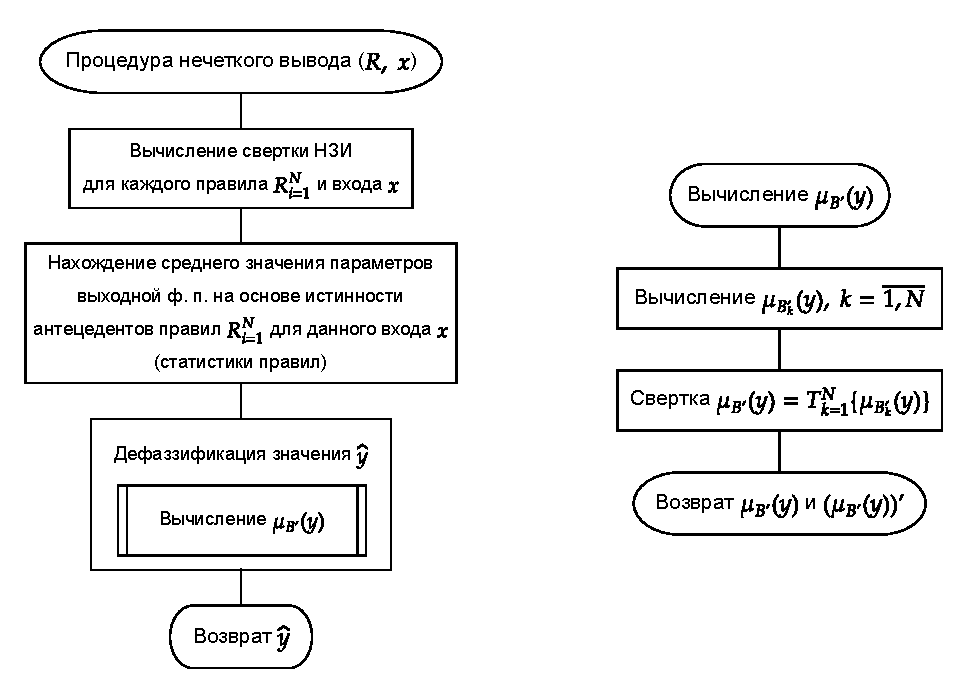
\includegraphics[scale=0.95]{fuzzy-infer-flowchart}
	\caption{Блок схема процедуры нечеткого логического вывода на основе нечеткого значения истинности.}
	\label{fig:fuzzy-infer-flowchart}
\end{figure}

При выполнении процедуры нечеткого вывода для набора входных данных можно выполнять процедуру вывода по каждому входному экземпляру независимо, то есть параллельно. Сам алгоритм нечеткого вывода не предусматривает наличия промежуточной информации, которой бы нужно было обмениваться между вычислениями по другим экземплярам входных данных. Тогда, поскольку алгоритм нечеткого вывода для каждого экземпляра входных данных можно реализовать при ограниченном небольшом объеме входных и промежуточных данных, имеет смысл разместить эти данные в памяти предоставляющей наибольшую скорость доступа к данным, которая в технологии CUDA соответствует разделяемой памяти внутри CUDA-блока, а сами вычисления над этими данными также реализовать внутри этого CUDA-блока.

Время нечеткого вывода может быть сокращено за счет уменьшения времени работы отдельного CUDA-блока путем увеличения количества параллельных CUDA-нитей. Тогда планировщик  \textit{потокового мультипроцессора} (\textit{streaming multiprocessor}) сможет распределять инструкции между доступными арифметико-логическими модулями, обеспечивая \textit{instruction pipelining}, или сократить амортизированное время задержки (\textit{latency}) при выполнении длительной инструкции подгрузки данных из глобальной памяти графического процессора. Однако с другой стороны слишком большое количество нитей внутри CUDA-блока упрется в ограниченное количество ригистровой памяти и ограниченное количество арифметико-логических модулей внутри потокового мультипроцессора (распределяемых между нитями 4-мя планировщиками на большинстве версий \textit{наборов вычислительных возможностей (compute capabilities)}. Ограниченность объема разделяемой памяти на один потоковый мультипроцессор также может ограничить предельное число CUDA-блоков, размещаемых в одном потоком мультипроцессоре, Согласно документации CUDA, устройства с набором вычислительных возможностей версии 7.5 (и некоторых более низких версий) максимальный объем разделяемой памяти на одном потоковом мультипроцессоре равен 64 Кб, а на устройствах с набором вычислительных возможностей более высокой версии --- предусмативается 100 - 164 Кб разделяемой памяти. Рациональное использование только необходимого объема разделяемой памяти позволит планировщику на графическом процессоре поставить на исполнение сразу несколько CUDA-блоков на один потоковый мультипроцессор.

\begin{figure}[ht]
	\centering
	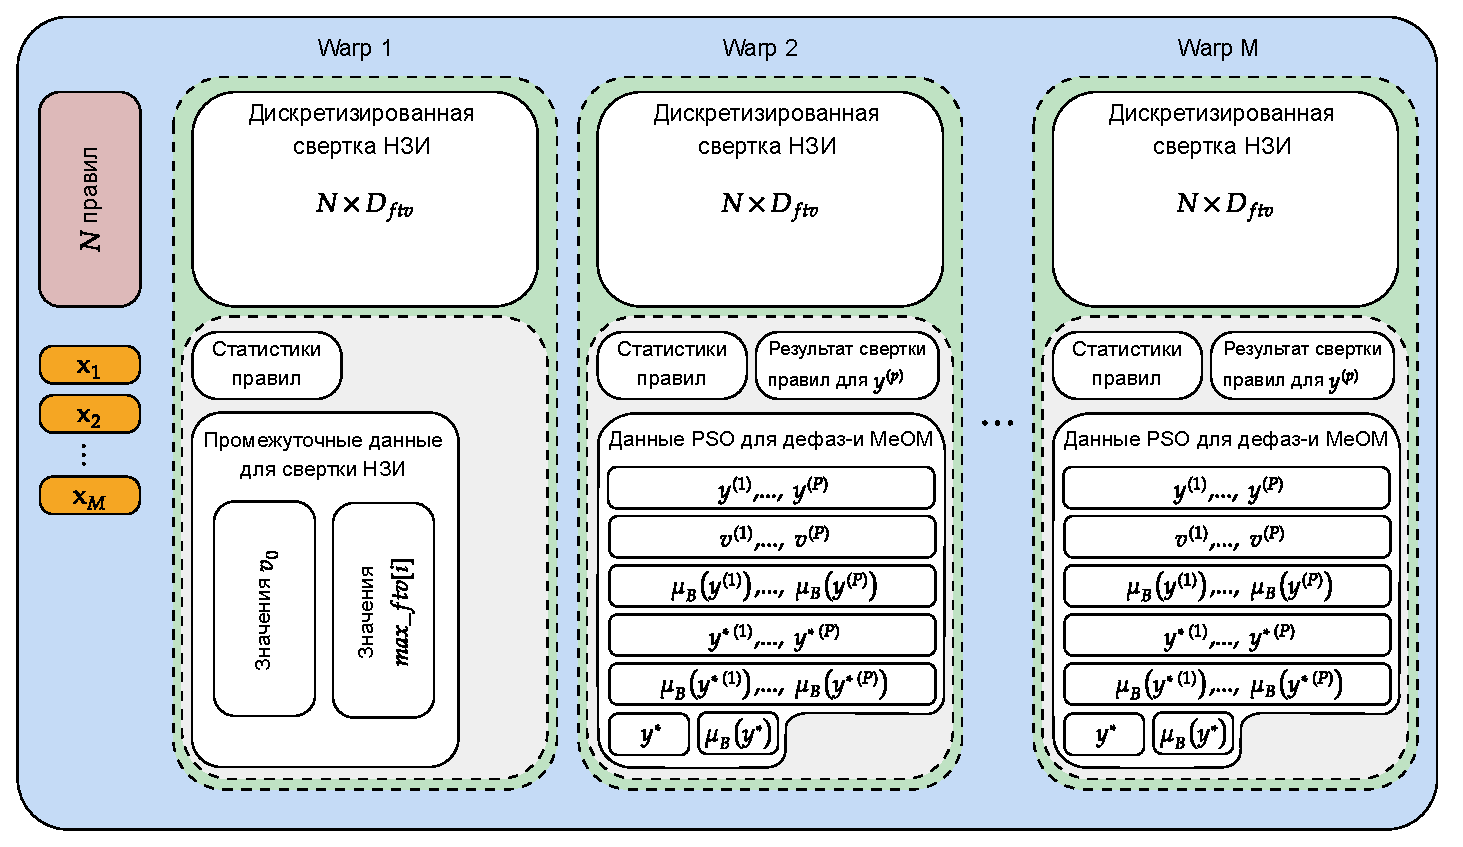
\includegraphics[scale=0.7]{cuda-shared-memory-map}
	\caption{Карта разделяемой памяти одного CUDA-блока нечеткого логического вывода на основе нечеткого значения истинности при использовании дефаззификации MeOM.}
	\label{fig:ftv-infer-cuda-shared-memory-map}
\end{figure}

Суммарный объем разделяемой памяти, необходимый для работы процедуры нечеткого вывода для одного входного экземпляра, складывается из объемов памяти используемых в этом выводе данных. Основной вклад в этот объем делают компоненты данных:
\begin{itemize}
	\item параметры ф. п. $N$ правил при $n$ входах (2 параметра для гауссовой ф-и): $(\text{\lstinline|sizeof float|}) \times (n+1) \times N \times 2$;
	\item параметры ф. п. входного экземпляра данных при $n$ входах (2 параметра для гауссовой ф-и): $(\text{\lstinline|sizeof float|}) \times (n+1) \times 2$;
	\item значения свертки НЗИ для $N$ правил при размере расчетной сетки равному $D_{ftv}$: $(\text{\lstinline|sizeof float|}) \times D_{ftv} \times N$ и промежуточные данные:
	\begin{itemize}
		\item индексы координат расчетной сетки с максимальным значением НЗИ каждому из $N$ правил и $n$ входов: $(\text{\lstinline|sizeof char|}) \times n \times N \times 2$;
		\item максимальные значения НЗИ на текущей итерации свертки НЗИ по каждому из $N$ правил и $n$ входов: $(\text{\lstinline|sizeof float|}) \times n \times N \times 2$;
	\end{itemize}
	\item популяции из $P$ координат $y^{(p)}$, скоростей изменения координат $v^{(p)}$, значений выходной ф. п. $\mu_{B'}(y^{(p)})$, координат локальных оптимумов $y^{*(p)}$, значений выходной ф. п. в локальных оптимумах $\mu_{B'}(y^{*(p)})$ (5 популяций): $(\text{\lstinline|sizeof float|}) \times P \times 5$.
\end{itemize}
Последний пункт приведен для случая использования \textit{MeOM} в качестве метода дефаззификации.

При нечетком выводе для одного входного экземпляра в одном CUDA-блоке, значимая доля вычислительного времени будет потрачена на загрузку базы правил из глобальной памяти в разделяемую память, а, в случае когда данные одного CUDA-блока будет занимать значимую долю доступной разделяемой памяти, число <<подменных>> CUDA-блоков на один потоковый процессор будет низким. Лучшим решением будет реализация <<долгоживущих>> CUDA-блоков, каждый из которых занимает большую часть разделяемой памяти. В таком случае база правил подгружается в разделяемую память один раз, а нечеткий вывод производится сразу для пакета экземпляров входных данных. Карта организации разделяемой памяти внутри одного такого CUDA-блока изображена на рисунке \cref{fig:ftv-infer-cuda-shared-memory-map}.

При достаточном размере пакета данных, обрабатываемых внутри одного CUDA-блока, нечеткий вывод по отдельному экземпляру выгодно реализовать внутри отдельного набора из 32-х нитей (\textit{warp}), которые исполняются единым пакетом нитей вычисления. Такой способ организации вычислений позволит практически полностью избавиться от барьерной синхронизации между нитями всего CUDA-блока с использованием \lstinline|__syncthreads()|, а для реализации эффективной свертки внутри набора из 32-х нитей CUDA предоставляет набор \textit{intrinsic}-функций --- \lstinline|__shfl()|, \lstinline|__shfl_down()|, \lstinline|__shfl_up()| и \lstinline|__shfl_xor()|.

Из описанного ранее функционала библиотеки Kokkos для размещения и доступа к данным в разделяемой памяти CUDA-блока крайне удобно использовать \lstinline|Kokkos::View| с опорой на широко эксплуатируемую в среде C++ разработчиков идиому RAII (Resource acquisition is initialization --- получение некоторого ресурса неразрывно совмещается с инициализацией, а освобождение --- с уничтожением объекта), которая позволяет избавиться от необходимости <<ручного>> вычисления адресов и смещений, располагаемых в разделяемой памяти, программных объектов, что особенно актуально при переиспользовании сегментов разделяемой памяти, занимаемых временными данными, в дальнейших шагах алгоритма.

Для удобства \dots

\begin{minted}[fontsize=\small,tabsize=4]{cpp}
using ScratchSpace =
	typename Kokkos::Cuda::scratch_memory_space;
template <typename DataType>
using ScratchView =
	Kokkos::View<DataType,
				 ScratchSpace,
				 Kokkos::MemoryTraits<Kokkos::Unmanaged>>;
\end{minted}

Для выделения памяти c помощью \lstinline|Kokkos::View| требуется получить дескриптор разделяемой памяти текущего CUDA-блока с помощью вызова \lstinline|Kokkos::TeamHandleConcept<>::team_shmem()| , который описывает текущее состояние разделяемой памяти данного CUDA-блока.

Поскольку вычисление свертки НЗИ для всех правил нечеткой системы составляет половину сложности алгоритма нечеткого вывода и в последствии будет неоднократно использооваться при агрегации правил, необходимо обеспечить единоразовое вычисление функции принадлежности свертки НЗИ (или ее аппроксимации), в результате которого будут известны значения последней на всей ее области определения.

\section{Вычисление нечеткого значения истинности посредством дискретизации}\label{sec:ch3/sect1}

При реализации вычисления НЗИ, когда функции принадлежности нечетких множеств $A$ и $A'$ заданы гауссовыми функциями, может возникнуть сложность, когда ф. п. НЗИ вырождается в близкий к некоторой асимптоте (горизонтальной или вертикальной) вид. Для изучения условий возникновения таких ситуаций перепишем формулу (\ref{eqn:ftv-gauss-expanded}) ниже и обозначим ее составные компоненты через $\alpha$, $\beta$, $\phi(v)$:
\begin{equation*}
	\exp\left(-\left(\underbrace{\frac{a_1-a_2}{b_2}}_{\alpha}\pm\underbrace{\frac{b_1}{b_2}}_{\beta}\underbrace{\sqrt{-\ln v}}_{\phi(v)}\right)^2\right).
	\label{eqn:ftv-gauss-components-markup}
\end{equation*}
Тогда вычисление значения (\ref{eqn:ftv-gauss-expanded}) можно представить в виде композиции функций
\begin{equation}
	\mu_{CP(A,A')}(v)=\exp(-z(v)^2),
	\label{eqn:ftv-gauss-exp-z}
\end{equation}
и
\begin{equation}
	z(v)=\alpha \pm \beta \phi(v).
	\label{eqn:ftv-gauss-phi}
\end{equation}

\pgfplotsset{
	membership axes/.style={
		%width=0.45\textwidth,
		%height=0.45\textwidth,
		scale only axis,
		domain=0:1,
		samples=100,
		every axis plot/.append style={smooth},
		axis lines=middle,
		xmin=0, xmax=1,
		ymin=0, ymax=1,
		xticklabel style={font=\tiny, inner sep=1pt, outer sep=0pt},
		yticklabel style={font=\tiny, inner sep=1pt, outer sep=0pt},
		legend style={font=\small},
	}
}


\begin{figure}[ht]
	\centering
	\begin{minipage}[t]{0.48\textwidth}
		\centering
		\begin{tikzpicture}
			\begin{axis}[
				membership axes,
				domain=0:5,
				samples=100,
				xmax=5,
			]
				\addplot [blue, thick] {exp(-(x^2))};
			\end{axis}
		\end{tikzpicture}
		\caption{График функции $\exp(-z^2)$}
		\label{fig:ftv-exp-component}
	\end{minipage}
	\hfill
	\begin{minipage}[t]{0.48\textwidth}
		\centering
		\begin{tikzpicture}
			\begin{axis}[
				membership axes,
				samples=100,
				ymax=3,
			]
				\addplot [blue, thick] {sqrt(-ln(x))};
			\end{axis}
		\end{tikzpicture}
		\caption{График функции $\phi(v)=\sqrt{-\ln v}$}
		\label{fig:ftv-phi-component}
	\end{minipage}
\end{figure}

Для иллюстрации условий возникновения описанных вырождений функции (\ref{eqn:ftv-gauss-expanded}) графики функций (\ref{eqn:ftv-gauss-exp-z}) и (\ref{eqn:ftv-gauss-phi}) при $\alpha = \beta = 1$ приведены на рисунках \cref{fig:ftv-exp-component} и \cref{fig:ftv-phi-component} соответственно. Из рисунка \cref{fig:ftv-phi-component} видно, что вырождение выражения (\ref{eqn:ftv-gauss-exp-z}) в близкий к асимптоте вид возможно при очень больших или очень малых значениях $\alpha$ и $\beta$. Данное наблюдение проиллюстрировано на рисунке \cref{fig:ftv-gauss-corner-cases}.

\begin{figure}[htbp]
	\centering
	
	% First row
	\begin{subfigure}[t]{0.48\textwidth}
		\newcommand{\aOne}{1}
		\newcommand{\bOne}{0.2}
		\newcommand{\aTwo}{0.95}
		\newcommand{\bTwo}{1}
		\centering
		\begin{tikzpicture}
			\begin{axis}[
				membership axes,
				samples=1000,
			]
				\addplot [blue, thick] {gauss(\aOne-2*\bOne*sqrt(-ln(x)), \aTwo, \bTwo)};
				\draw [blue, thick] (0.001464278918,0.8) -- (0.0001,0);
			\end{axis}
		\end{tikzpicture}
		\caption{$\mu_{CP(A, A')}(v)$ при $\alpha \approx 0, \beta \approx 0$}
		\label{fig:ftv-corner-cases-zeroBeta-1}
	\end{subfigure}
	\hfill
	\begin{subfigure}[t]{0.48\textwidth}
		\newcommand{\aOne}{1}
		\newcommand{\bOne}{1}
		\newcommand{\aTwo}{0.95}
		\newcommand{\bTwo}{0.1}
		\centering
		\begin{tikzpicture}
			\begin{axis}[
				membership axes,
				samples=1000,
			]
				\addplot [blue, thick] {gauss(\aOne-2*\bOne*sqrt(-ln(x)), \aTwo, \bTwo)};
			\end{axis}
		\end{tikzpicture}
		\caption{$\mu_{CP(A, A')}(v)$ при $\alpha \approx 0, \beta \gg 0$}
		\label{fig:ftv-corner-cases-largeBeta-1}
	\end{subfigure}
	
	% Second row
	\begin{subfigure}[t]{0.48\textwidth}
		\newcommand{\aOne}{3.34}
		\newcommand{\bOne}{0.02}
		\newcommand{\aTwo}{5}
		\newcommand{\bTwo}{1}
		\centering
		\begin{tikzpicture}
			\begin{axis}[
				membership axes,
				samples=1000,
				domain=0.001:1,
			]
				\addplot [blue, thick] {gauss(\aOne+2*\bOne*sqrt(-ln(x)), \aTwo, \bTwo)};
			\end{axis}
		\end{tikzpicture}
		\caption{$\mu_{CP(A, A')}(v)$ при $|\alpha| \gg 0, \beta \approx 0$}
		\label{fig:ftv-corner-cases-zeroBeta-2}
	\end{subfigure}
	\hfill
	\begin{subfigure}[t]{0.48\textwidth}
		\newcommand{\aOne}{3.34}
		\newcommand{\bOne}{1}
		\newcommand{\aTwo}{5}
		\newcommand{\bTwo}{0.02}
		\centering
		\begin{tikzpicture}
			\begin{axis}[
				membership axes,
				samples=1000,
				domain=0.001:1,
			]
				\addplot [blue, thick] {gauss(\aOne+2*\bOne*sqrt(-ln(x)), \aTwo, \bTwo)};
			\end{axis}
		\end{tikzpicture}
		\caption{$\mu_{CP(A, A')}(v)$ при $|\alpha| \gg 0, \beta \gg 0$}
		\label{fig:ftv-corner-cases-largeBeta-2}
	\end{subfigure}
	
	% Third row
	\begin{subfigure}[t]{0.48\textwidth}
		\newcommand{\aOne}{1}
		\newcommand{\bOne}{0.1}
		\newcommand{\aTwo}{0.3}
		\newcommand{\bTwo}{0.1}
		\centering
		\begin{tikzpicture}
			\begin{axis}[
				membership axes,
				samples=1000,
			]
				\addplot [blue, thick] {gauss(\aOne-2*\bOne*sqrt(-ln(x)), \aTwo, \bTwo)};
				\draw [blue, thick] (0.0014,0.4) -- (0.0001,1);
			\end{axis}
		\end{tikzpicture}
		\caption{$\mu_{CP(A, A')}(v)$ при $|\alpha| \gg 0, \beta = 1$}
		\label{fig:ftv-corner-cases-oneBeta}
	\end{subfigure}
	
	\caption{Случаи вырождения ф. п. НЗИ в близкий к асимптоте вид.}
	\label{fig:ftv-gauss-corner-cases}
\end{figure}

В ситуациях, изображенных на рисунках \cref{fig:ftv-corner-cases-zeroBeta-1, fig:ftv-corner-cases-largeBeta-1, fig:ftv-corner-cases-largeBeta-2, fig:ftv-corner-cases-oneBeta}, функция принадлежности НЗИ имеет своей асимптотой вертикальную прямую $v = v_0$. При реализации вычисления НЗИ с использованием расчетной сетки, связанная с тем, что ф. п. НЗИ в точке может быть вообще не определена (рис. \cref{fig:ftv-corner-cases-zeroBeta-1, fig:ftv-corner-cases-oneBeta}) или ф. п. НЗИ в точке $v_0$ имеет значение сильно отличающееся от значений в ближайших точках расчетной сетки $v_1$ и $v_2$ при $v_0 \in (v_1, v_2)$, из-за чего значение НЗИ в бесконечно малой окрестности точки $v_0$ будет упущено.

Из рисунка \cref{fig:ftv-exp-component} видно, что максимальное значение выражения (\ref{eqn:ftv-gauss-exp-z}), равное 1, достигается при $z = 0$, а из рисунка \cref{fig:ftv-phi-component} видно, что функция (\ref{eqn:ftv-gauss-phi}) обязательно пересекает ось абсцисс, то есть максимальное значение ф. п. НЗИ всегда равно 1. Тогда для решения проблемы <<просеивания>> значения $\mu_{CP(A, A')}(v_0)$ сквозь точки расчетной сетки можно вычислить координату точки $v_0$, в которой функция (\ref{eqn:ftv-gauss-expanded}) принимает свое максимальное значение, а затем положить значение в ближайшей к $v_0$ точке расчетной сетки равным этому максимуму, то есть значению 1. Для этого выразим аналитически значение $v_0$, в котором (\ref{eqn:ftv-gauss-expanded}) принимает значение 1.

\begin{align}
	\exp\left(-\left(\frac{(a_1-a_2)\pm b_1\sqrt{-\ln v_0}}{b_2}\right)^2\right) &= 1 \nonumber \\
	\exp\left(-\left(\frac{(a_1-a_2)\pm b_1\sqrt{-\ln v_0}}{b_2}\right)^2\right) &= \exp(0) \nonumber \\
	\frac{(a_1-a_2)\pm b_1\sqrt{-\ln v_0}}{b_2} &= 0 \nonumber \\
	\pm b_1\sqrt{-\ln v_0} &= a_1-a_2 \nonumber \\
	\sqrt{-\ln v_0} &= \pm\frac{a_1-a_2}{b_1} \nonumber \\
	\ln v_0 &= -\left(\frac{a_1-a_2}{b_1}\right)^2 \nonumber \\
	v_0 &= \exp\left(-\left(\frac{a_1-a_2}{b_1}\right)^2\right) \label{eqn:ftv-gauss-argmax}
\end{align}

Внедрение выражения (\ref{eqn:ftv-gauss-argmax}) в алгоритм вычисления НЗИ позволит обеспечить соответствие определению дискретизированного представления ф. п. НЗИ. \todo{Строго говоря ф. п. на рисунке определена в точке $v_0$ и не требует\dots.} НЗИ с функцией принадлежности, имеющей горизонтальную асимптоту, как на рисунке \cref{fig:ftv-corner-cases-zeroBeta-2} может вызвать сложность при построении алгоритма вычисления НЗИ на использовании метода градиентного спуска вместо дискретизации с фиксированным шагом расчетной сетки.

Вычисление нечеткого значения истинности для каждого правила по каждому входу отдельно предварительным этапом приведет к линейному увеличению объема необходимой памяти. Поскольку вычисление НЗИ является довольно легкой операцией, лучшим решением будет встраивание вычисления НЗИ по каждому входу в процедуру свертки НЗИ.

Формула (\ref{}) предлагает построение процедуры свертки НЗИ в виде дерева попарных сверток, для сохранения промежуточных результатов которых потребуется выделение объема памяти, также имеющего фактически линейный порядок зависимости от количества входов нечеткой системы. Возвращаясь к формуле (\ref{}) свертки НЗИ по входам в [] предложен параллельный алгоритм свертки НЗИ на расчетной сетке с постоянным шагом. Данный алгоритм итеративно вычисляет значение свертки НЗИ в каждой точки расчетной сетки продвигаясь от точки в пространстве истинности 1 к точке 0. Для каждого правила отдельно потребуется объем памяти, необходимый для сохранения значений свертки НЗИ в каждой точке расчетной сетки и для сохранения текущего максимального значения НЗИ по каждому входу на данной итерации алгоритма.

Преимуществом такого подхода представления НЗИ в программе является возможность быстрого нахождения значения функции принадлжености НЗИ в некоторой точке пространства истинности. Пара ближайших к этой точке позиций в массиве значений НЗИ на расчетной сетке определяется на основе значения фиксированного шага расчетной сетки. Для вычисления непосредственно ззначения НЗИ используется линейная интерполяция для найденной пары.

Поскольку при небольшом количестве входных переменных нечеткой системы большие участки расчетной сетки ф. п. свертки НЗИ соответствуют ф. п. НЗИ по одному из входов, при том же объеме памяти, необходимой для хранения результа сверки НЗИ, можно перейти к переменному шагу расчетной сетки с увеличением сложности функции аппроксимации участков ф. п. свертки НЗИ, принадлежащий ф. п. НЗИ одного из входов. Схема вычислений такого алгоритма схожа со схемой алгоритма при использовании постоянного шага расчетной сетки, а на каждой итерации определяется точка \dots

Ввиду необходимости использования большой размерности расчетной сетки для получения высокой точности дискретизации для размещения результата свертки НЗИ потребуется существенный объем разделяемой памяти. Например, при использовании для задания вычисленных значений вещественных чисел одинарной точности (4 байта) и размерности расчетной сетки равной 100 сохранение результата свертки НЗИ в нечеткой системе с 50 правилами в базе правил потребуется $4\textrm{ байта}\times 100 \times 50 = 20000\textrm{ байт}$ разделяемой памяти.

\begin{figure}[hbt]
	\centering
   	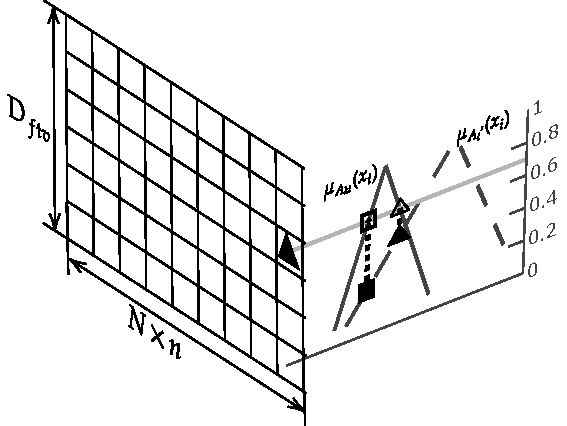
\includegraphics[width=0.6\textwidth]{ftv-opengl-computation.pdf}
	\label{ftv-opengl-computation}
\end{figure}

\begin{figure}[hbt]
	\centering
   	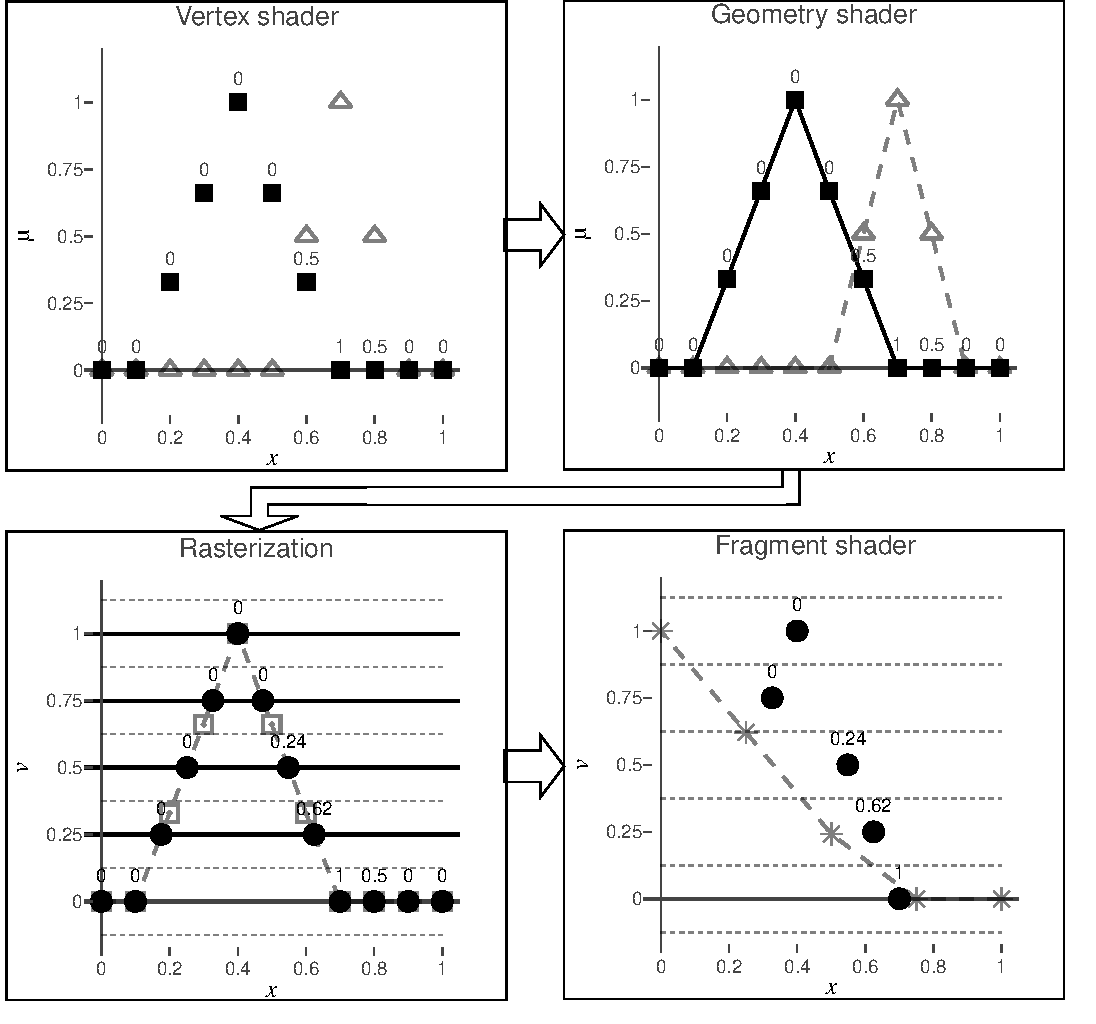
\includegraphics[width=1.0\textwidth]{ftv-opengl-computation-pipeline.pdf}
	\label{ftv-opengl-computation-pipeline}
\end{figure}

\section{Алгоритм свертки НЗИ при $T_1=min$ и $T_3$ - неубывающая по всем аргументам}\label{sec:ch3/sect2}

При дискретизированном вычисление ф. п. свертки НЗИ в некоторой точке расчетной сетки $v_j\in [0,1]$ потребуется просматривать значения НЗИ в отрезке $[v_j, 1]$, то есть имеет вычислительную сложность $O(D_{ftv})$, где $D_{ftv}$ --- число точек расчетной сетки ф. п. НЗИ. Таким образом вычисление свертки НЗИ по формуле (\ref{eqn:ftv-compute-11}) может быть распараллелено по точкам расчетной сетки, а нахождение $\tau_{\mathbf{A_k}|\mathbf{A'}}(v_j)$ использует операцию свертки, которая в имеет ограниченную возможность распараллеливания, но в целом требует большого количества повторных вычислений значений $\tau_{A_{ki}|A'_i}(v_k), v_k\in [v_j, 1]$. В \cite{Karatach2024} предложен алгоритм вычисления свертки НЗИ сразу по всем входам с использованием техники динамического программирования, имеющий линейную зависимость от размера расчетной сетки $D_{ftv}$. Алгоритм приведен на \cref{alg:ftv-reduction}.

\begin{algorithm}
\begin{algorithmic}
\Require $ftv_i,\ i=\overline{1,n}$
\State $max\_ftv[i] = 0;$
\For{$v_j = 1\dots0$}
\State $s \gets \left\{ftv_i[v_j] \mid ftv_i[v_j] >= max\_ftv[i]\right\};$
\State $max\_ftv[i] \gets max(max\_ftv[i], ftv_i[v_j]);$
\State $v\_max \gets \max_{i}\left\{ftv_i[v_j]\right\}, v\_max\_index \gets \mathrm{arg\,max}_i\left\{ftv_i[v_j]\right\};$
\If{$s = \emptyset \And i = v\_max\_index$}
\State $r[i] \gets v\_max;$
\Else
\State $r[i] \gets max\_ftv[i];$
\EndIf
\State $ftv'[v_j] \gets \underset{i}{T_3}\left\{r[i]\right\}$;
\EndFor
\State \Return $ftv'$
\end{algorithmic}
\caption{Алгоритм свертки НЗИ при $T_1=min$ и $T_3(a, b) \ge T_3(c, d)$ если $a > c$ или $b > d$}
\label{alg:ftv-reduction}
\end{algorithm}

Данный алгоритм итеративно вычисляет значения $\tau_{\mathbf{A_k}|\mathbf{A'}}(v_j)$, продвигаясь от точки $v_j = 1$ к $v_j = 0$. При этом распараллеливаются вычисления по $n$ входам. В $i$-х элементах массива $max\_ftv$ хранятся максимальные значения $\tau_{A_{ki}|A'_i}(v_k)$ для $j$-й итерации, что избавляет от необходимости поиска этих значений на каждой итерации. Также, поскольку на $j$-й итерации значение $\tau_{\mathbf{A_k}|\mathbf{A'}}(v_j)$ выражается из значений НЗИ по входам в точках $v_{ki}, i=\overline{1,n}$, то, с учетом ограничения алгоритма $T_1 = min$ и согласно выражению из формулы (\ref{eqn:ftv-compute-8})
\[
\underset{i=\overline{1,n}}{\mathrm{T_1}}v_{ki} = v_j,
%\sup_{\substack{\underset{i=\overline{1,n}}{\mathrm{T_1}}v_i = v \\ (v_1, \dots, v_n) \in [0, 1]^n}} \left\{\underset{i=\overline{1,n}}{\mathrm{T_3}}\tau_{A_{ki}|A'_i}(v_i)\right\}
\]
для одного из значений $v_{ki}$ необходимо выполнение $V_{ki} = v_j$. Для этого в \cref{alg:ftv-reduction} используется максимальное значение $\tau_{A_{ki}|A'_i}(v_j), i=\overline{1,n}$, когда ни по одному входу не обнаружено нового максимума ф. п. НЗИ в точке $v_j$.

Для лучшего понимания работа алгоритма на каждой итерации изображена на рисунке \cref{fig:ftvs-reduction-example}. %, в центре диаграммы находится координата осей равная 1, а сама <<роза>> проходит через текущие максимумы ф. п. НЗИ на отрезке $[v_j, 1]$.

\begin{figure}
    \label{fig:ftvs-reduction-example}
    \centering
    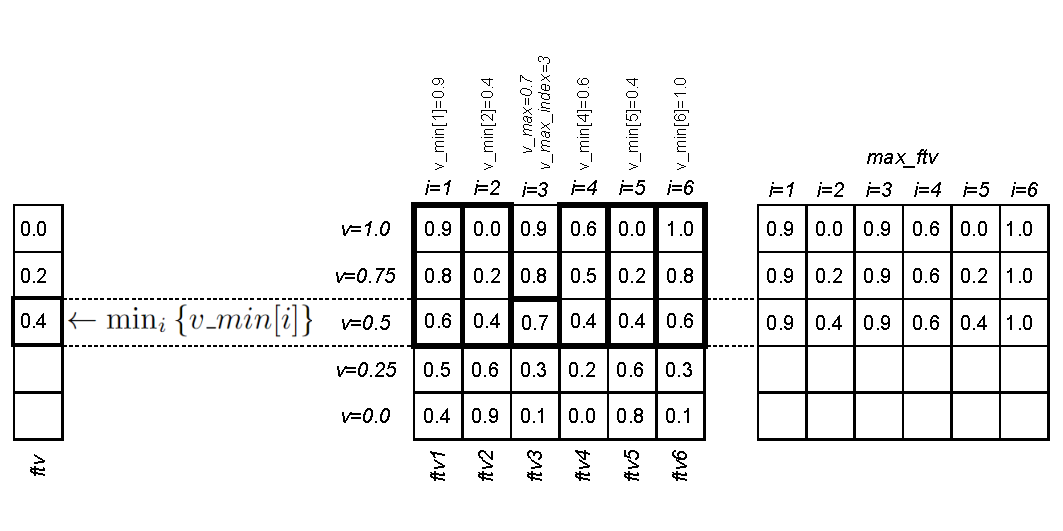
\includegraphics[width=15cm]{ftvs-reduction-example.pdf}
    \caption{Иллюстрация работы алгоритма свертки НЗИ для нескольких входов для расширенной $\mathrm{\tilde{T}}$-нормы при $T_1=\mathrm{min}$ и $T_3=\mathrm{min}$.}
\end{figure}

При 

\pgfplotsset{
    axis grid/.style={
        width=0.3\textwidth,
        height=0.3\textwidth,
        domain=0:1,
    }
}


\section{Реализация дефаззификации}

Производительность дефаззификации по \textit{упрощенной схеме метода COG} может быть увеличена путем масштабирования вычислений внутри блока по центрам выходной лингвистической переменной.

Поскольку используемые в данной работе в качестве функций принадлежности гауссовы функции являются гладкими во всей области определения выходной лингвистической переменной, для точного нахождения максимального значения ф. п. выходного нечеткого множества при дефаззификации по \textit{методу среднего максимума (MeOM)} можно использовать алгоритм градиентного спуска. В ситуации когда вычисление значения агрегированной по всем правилам выходной функции принадлежности и ее производных в некоторой точке выходного пространства является вычислительно сложной процедурой, целесообразно будет использовать \textit{метод Ньютона второго порядка} для более быстрого нахождения точки максимума выходной ф. п.:
\begin{equation}
	y^{(k+1)} = y^{(k)} - \alpha \frac{\mu_{B'}^{'}(y^{(k)})}{\mu_{B'}^{''}(y^{(k)})},
	\label{eqn:defuz-impl-meom-1}
\end{equation}
где $\alpha $ - коэффициент шага градиента.

Сложность может составить вопрос инициализации начальной координаты точки $y^{(0)}$, ведь в отдаленных от точки максимума выходной ф. п. $\mu_{B'}(y^{(0)})$  соответствующая ее минимуму гауссова функция может принять горизонтальный вид с нулевыми производными вне границ отрезка $[a_{B'} - 4 b_{B'}, a_{B'} + 4 b_{B'}]$. Для получения начального приближения можно использовать вычислительно более простой метод дефаззификации, например, дефаззификацию по методу среднего центра (CA). Также стоит добавить в формулу (\ref{eqn:defuz-impl-meom-1}) штраф за отдаление от точки $\hat{y}_{CA}$ с весовым параметром учета штрафа $\lambda$, а также учитывать штраф при низких значениях $\mu_{B'}(y^{(k)})$. С помощью параметра $\lambda$ и номера итерации $k$ можно обеспечить плавный сдвиг вклада в шаг итерации от штрафа до значения градиента с ростом числа прошедших итераций. Тогда формула (\ref{eqn:defuz-impl-meom-1}) примет вид:
\begin{gather*}
	y^{(k+1)} = y^{(k)} + \alpha \left(\mu_{B'}(y^{(k)})(1-\lambda)\left(-\frac{\mu_{B'}^{'}(y^{(k)})}{\mu_{B'}^{''}(y^{(k)})}\right) + (1-\mu_{B'}(y^{(k)}))\lambda (\hat{y}_{CA} - y^{(k)})\right),\\
	\lambda = e^{-k \gamma},
	\label{eqn:defuz-impl-meom-2}
\end{gather*}
где хорошая сходимость алгоритма показывается при выборе для параметра $\gamma$ значения равного коэффициенту шага $\alpha$.

Для преодоления проблемы локальных максимумов выходной функции принадлежности (которые ожидаемо возникнут при использовании $t$-нормы минимума или произведения для агрегации гауссовых функций) и сглаживания линии градиента, распространенной практикой является добавление момента $v^(k)$ в алгоритм градиентного спуска:
\begin{gather}
\begin{split}
	v^{(k+1)} = \omega v^{(k)} + (\mu_{B'}(y^{(k)})(1-\lambda)\left(-\frac{\mu_{B'}^{'}(y^{(k)})}{\mu_{B'}^{''}(y^{(k)})}\right) + (1-\mu_{B'}(y^{(k)}))\lambda (\hat{y}_{CA} - y^{(k)})),\\
	y^{(k+1)} = y^{(k)} + \alpha v^{(k+1)},
\end{split}
\label{eqn:defuz-impl-meom-3}
\end{gather}
где $\omega$ --- параметр скользящего среднего значения момента.

\begin{figure}[ht]
	\centering
	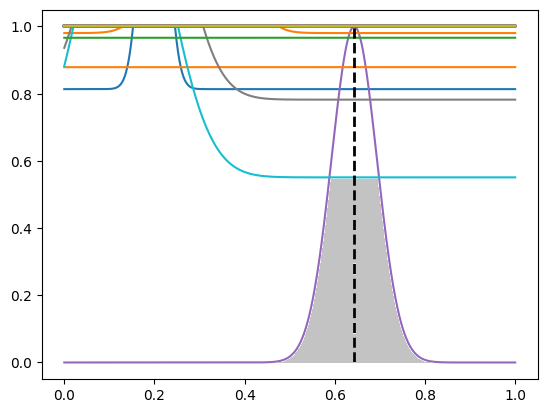
\includegraphics{meom-use-case.png}
	\caption{Ситуация необходимости нахождения среднего максимума при дефаззификации агрегированной функции принадлежности $\mu_{B'}(y)$.}
	\label{fig:defuz-meom-use-case}	
\end{figure}

Необходимость усреднения максимумов при использовании метода дефаззификации Mean of Maximum возникает в ситуации изображенной на рисунке \cref{fig:defuz-meom-use-case}, где истинное значение $y$ нарисовано пунктирной линией. Вычислить среднее значение $y$ можно как выборочное среднее. Получить такую выборку точек можно посредством многократной оптимизации описанном выше методом. Как и в случае с упрощенной схемой дефаззификации каждая такая оптимизация может происходить в отдельной группе нитей (warps) за счет масштабирования одного CUDA-блока.

Для этого можно использовать один из методов глобальной оптимизации, например, \textit{Gradient-aware Particle Swarm Optimizatiion}. Метод Particle Swarm Optimization (PSO) обеспечивает синхронизацию информации о текущей глобальной точке оптимума на данной итерации внутри популяции точек, что сокращает число итерации до сходимости к максимальному значению выходной функции принадлежности. С учетом (\ref{eqn:defuz-impl-meom-3}) для данного метода формулы шага оптимизации можно составить следующим образом:
\begin{align}
	\begin{split}
		v_i^{(k+1)} &= \omega v_i^{(k)} +\\
		&+ \alpha_l \left(
			r_l\left(
				y_i^{best} - y_i^{(k)}
			\right) + (1-r_l)\left(
				-\frac{\mu_{B'}^{'}(y_i^{(k)})}{\mu_{B'}^{''}(y_i^{(k)})}
			\right)
		\right) + \\
		&+ \alpha_g \left(
			r_g \mu_{B'}(y^{best})\left(
				y^{best}-y
			\right) + (1-r_g) \left(
				1-\mu_{B'}(y^{best})
			\right) \left(
				\hat{y}_{CA} - y^{(k)}
			\right)
		\right), \label{eqn:defuz-impl-meom-4-1}
	\end{split}\\
	y^{(k+1)} &= y^{(k)} + v^{(k+1)}, \nonumber
\end{align}
где $\alpha_l$ и $\alpha_g$ --- коэффициенты шага в направлении текущей точки локального и глобального оптимума, $r_l$ и $r_g$ --- случайно сгенерированные числа в диапазоне $[0,1]$, параметризующие движение в сторону текущих точек локального и глобального оптимума алгоритма PSO между движением в сторону роста градиента и точки начального приближения $\hat{y}_{CA}$ соответственно.

\begin{figure}[ht]
	\centering
	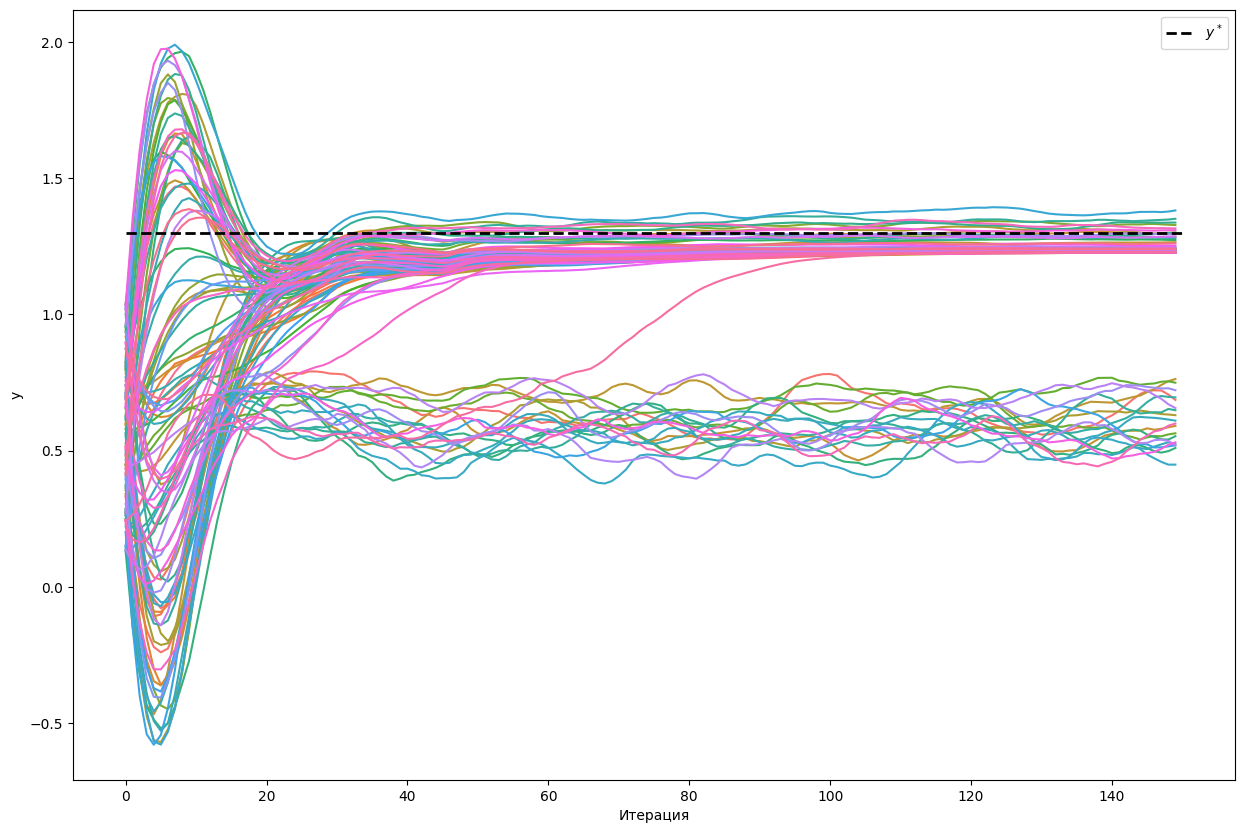
\includegraphics[scale=0.55]{defuz-meom-pos-hue.png}
	%	\hfill
	%	\begin{subfigure}{0.5\textwidth}
		%		\centering
		%		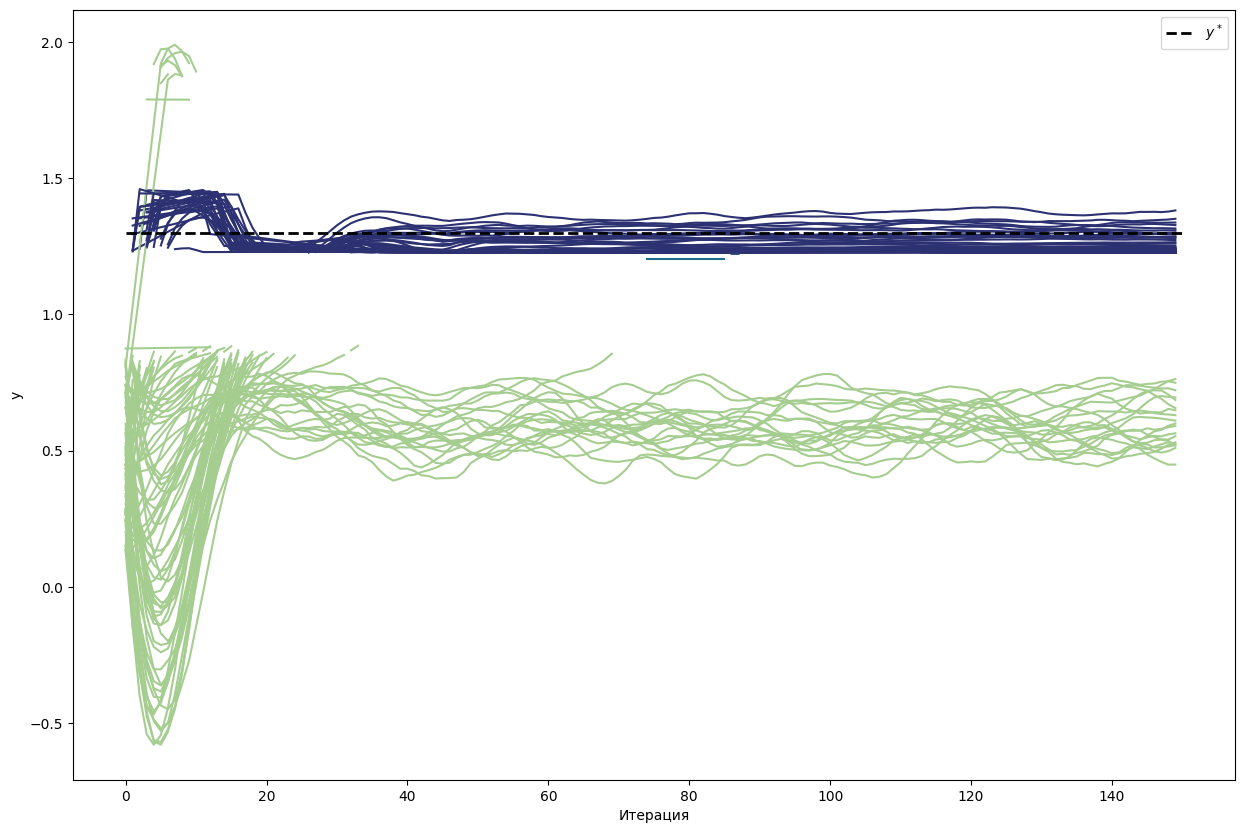
\includegraphics{defuz-meom-pos-brightness.png}
		%	\end{subfigure}
	\caption{Динамика движения точек популяции при работе алгоритма глобальной оптимизации Gradient-aware PSO.}
	\label{fig:defuz-meom-pso-hue}
\end{figure}

Компонента после коэффициента $\alpha_l$ в формуле (\ref{eqn:defuz-impl-meom-4-1}) обеспечить разнообразие среди точек популяции, достигших максимума $\mu_{B'}(y_i^{(k)})$. График работы такого алгоритма PSO приведен на рисунке \cref{fig:defuz-meom-pso-hue}. Как видно из него --- большинство точек популяции сосредоточились возле точки оптимума.

Для реализации дефаззификации по \textit{методу центра тяжести} можно использовать алгоритм оптимизации из предыдущего метода, сохраняя координаты $y_i^{(k)}$ и значения $\mu_{B'}(y_i^{(k)})$ на каждой итерации, а затем для вычисления формулы (\ref{eqn:defuz-cog-2}) использовать численное интегрирование, например, методом Симпсона.

\section{Ускорение вывода за счет фильтрации ближайших правил}%\label{sec:ch3/sect2}

Как описано в разделе \ref{}, на основе рисунка \cref{fig:out_mf_with_low_crossing} и графика истинности отмечается отсутствие необходимости включать в процедуру вывода для данного входа весь набор правил из базы правил, поскольку в случае отсутствия пересечения входных нечетких множеств и нечетких множеств антецедента, центроида НЗИ будет около 0, а ф. п. отношения импликации тогда примет значение равное 1 независимо от значения ф. п. консеквента. При использовании для сверки правил $t$-нормы из свойства $T(a, 1) = a$ вытекает отсутствие необходимости включать такие правила в процедуру свертки правил, что способно значительно сократить время выполнения процедуры нечеткого вывода, особенно при использовании методов дефаззификации, предполагающих множество сверток правил при нахождения $\mu_{B'}(y)$ для оптимизацию значения $\hat{y}$.

Для этого предлагается включать в процедуру вывода $K$ правил с наибольшим значением истинности по отношению к данному входу. Поскольку вычисление НЗИ в свою очередь является вычислительно сложной процедурой, в качестве эвристики предлагается использовать одну из мер расстояния между нечеткими множествами. В качестве меры совместимости нечетких множеств $\mu_{A_1}(x)$ и $\mu_{A_2}(x)$ можно использовать дополнение до единицы \textit{нормированное Евклидово расстояние} гауссовых функций принадлежности $g_1(x; a, b)$ и $g_2(x; a, b)$ этих нечетких множеств, которое выражается формулой:

\begin{align*}
	\rho(A_1, A_2) = ||g_1 - g_2|| &= \sqrt{\int_{-\infty}^{\infty} \left(g_1(x) - g_2(x)\right)^2 dx} \\
	&= \sqrt{\int_{-\infty}^{\infty} g_1^2 + \int_{-\infty}^{\infty} g_2^2 - 2\int_{-\infty}^{\infty} \todo{g_1^2 g_2^2}}\\
	\int_{-\infty}^{\infty} g_1^2(x) dx &= b_1 \sqrt{\pi}\\
	\int_{-\infty}^{\infty} g_2^2(x) dx &= b_2 \sqrt{\pi}\\
	\int_{-\infty}^{\infty} \todo{g_1^2(x) g_2^2(x)} dx &= \sqrt{\frac{2\pi b_1^2 b_2^2}{b_1^2+b_2^2}} \exp\left(-\left(\frac{(a_1-a_2)^2}{2(b_1^2+b_2^2)}\right)\right)
\end{align*}

Для многомерного случая мера совместимости:
\begin{equation*}
	\rho(\mathbf{A_1}, \mathbf{A_2}) = 1 - \sqrt{\frac{1}{n} \sum_{i=1}^{n} \rho(A_{1i}, A_{2i})}
\end{equation*}
где $n$ --- размерность нечетких множеств $A_1$ и $A_1$.

Помимо более простого способа оценки схожести входных н. м. и н. м. антецедента следует обеспечить эффективный способ нахождения $K$ правил с наибольшей схожестью.

\begin{figure}[hbt]
	\label{fig:z-curve-apetrei}
	\centering
	\begin{minipage}[b]{0.45\textwidth}
		\centering
		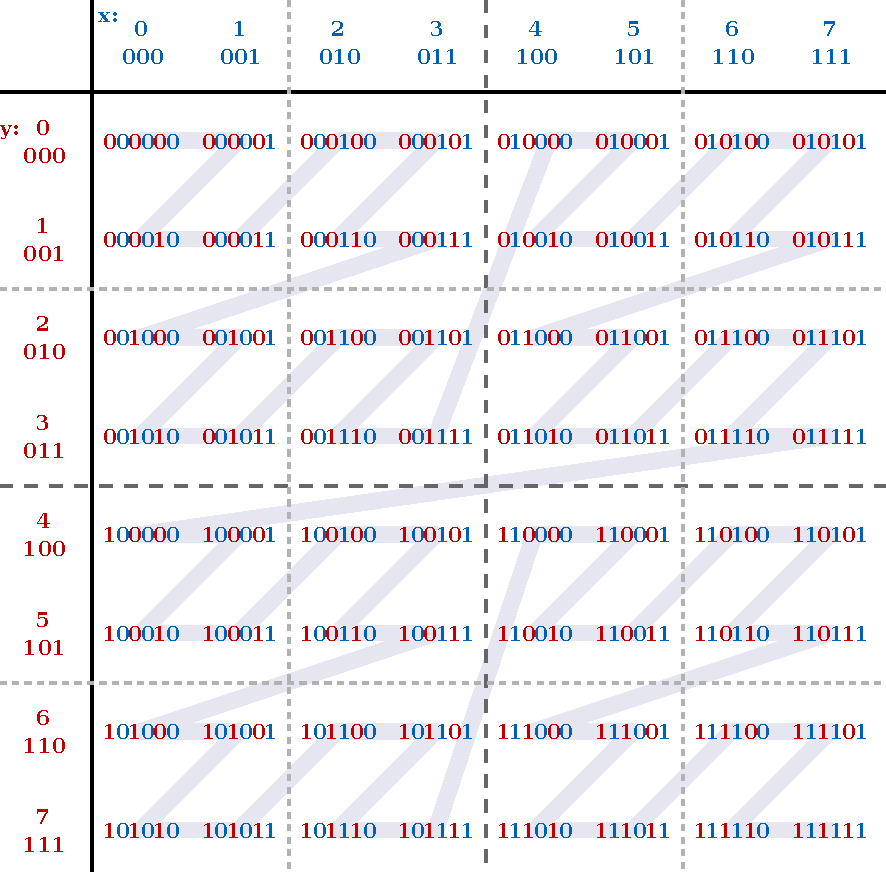
\includegraphics[width=\textwidth]{z-curve}
		\caption*{(a) z-curve}
	\end{minipage}\hfill
	\begin{minipage}[b]{0.45\textwidth}
		\centering
		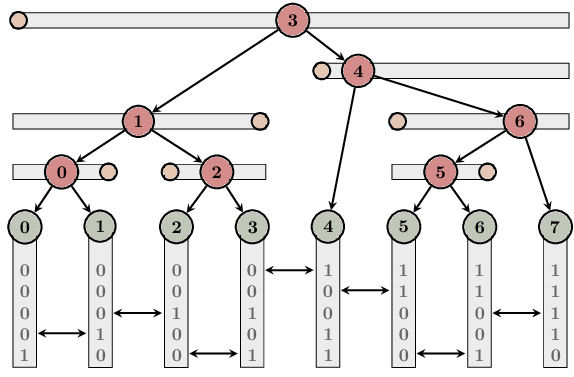
\includegraphics[width=\textwidth]{apetrei}
		\caption*{(b) apetrei}
	\end{minipage}
	\caption{Две иллюстрации: графика z-curve и apetrei.}
\end{figure}

В \cite{prokopenko2024revisingapetreisboundingvolume} авторами библиотеки \textbf{ArborX} предложен алгоритм для эффективного построения \textit{иерархии ограничивающих объемов}. Данная структура данных используется для эффективного поиска ближайшей точки в $n$-мерном пространстве. Алгоритм выполняет построение структуры поиска за $O(N\times log(N))$, где $N$ - количество точек в исходном наборе. Логика поиска места в иерархии ограничивающих объемов для каждой отдельной точки помещена в отдельную нить параллельных вычислений, после чего остается только логирифмическая компонента сложности, соответствующая восходящему обходу промежуточного дерева и помещения точки в подобранный узел \fixme{с использованием атомарной операции}. В основе алгоритма лежит группировка близко расположенных точек для более быстрого подбора соответствующего ограничивающего объема за счет проецирования точки из $n$-мерного пространства на $Z$-кривую посредством вычисления кода Мортона для каждой точки. Согласно эвристике, лежащие рядом на $Z$-кривой точки располагаются достаточно близко и исходном $n$-мерном пространстве. Кроме того в статье описан модифицированный алгоритм Апетрея [], обеспечивающий обход иерархии на этапе поиска ближайших точек без необходимости помещения цепочки пройденных родительских узлов в стек за счет передачи информации об альтернативных узлах-кандидатах из родительских узлов в дочерние. Такой подход значительно снижает количество потребляемой памяти для сохранения промежуточной информации при выполнении этапа поиска.

\todo{Однако при таком подходе не получится}

\section{Реализация алгоритма построения базы правил}

Для оценки предельного качества предложенного метода нечеткого вывода важно обеспечить метод нахождения оптимальной структуры правил, при которой нечеткая модель достигает максимального качества моделирования набора данных. Оптимизация базы правил позволяет оценить непосредственно качество моделирования, исключая неоптимальность извлечения знаний из набора данных, как при построении базы правил на основе эталонов. Поскольку композиция операций описанной в работе нейро-нечеткой системы не является гладкой функцией (например, при использовании $t$-нормы $min$), для выполнения оптимизации не подходят методы градиентного спуска. В такой ситуации следует использовать методы глобальной оптимизации, представителем которых являются семейство алгоритмов оптимизации на основе роевого интеллекта. Одним из них является мета эвристический алгоритм \textit{метод роя частиц (particle swarm optimization, PSO)} \cite{Kennedy1995}.

В отличие от градиентного спуска, PSO не нуждается в вычислении производных ошибки. Частицы в PSO используют как собственный опыт, так и опыт соседей. Это позволяет алгоритму избегать застревания в локальных минимумах. В контексте оптимизации вектора параметров функций принадлежности базы правил большой размерности (часто, сотни параметров), PSO хорошо выполняет оптимизацию по всем размерностям одновременно. При работе алгоритм сперва исследует широкое пространство решений, а затем сосредоточиться на его уточнении, что также позволяет бороться с попаданием в локальный оптимум. Основные параметры --- количество частиц, вес инерции $\omega$ и коэффициенты влияния локального $\phi_l$ и глобального $\phi_g$ оптимума. \todo{Частицы работают независимо, а вычисление функции приспособленности можно выполнять параллельно. Данный метод часто применяется для оптимизации нейро-нечетких систем в литературе.}

В выполненной реализации для утилизации параллелизма графического ускорителя основная часть вычислений была перенесена внутрь CUDA-ядер. Например, вычисление функции приспособленности по каждой точке популяции производилось в отдельном CUDA-блоке. Для этого популяции частиц, вектора скорости и соответствующих оценки функции приспособленности были размещены в памяти графического устройстве, а копирование в память хоста минимизировано до объема данных, необходимых для формирования аргументов CUDA-ядер шагов данного алгоритма.

\section{Реализация обертки в Python-модуль}

Для ускорения процесса отладки и тестирования, выполненная на языке C++ (CUDA) реализация нечеткой модели собирается компилятором NVCC в динамически подключаемую библиотеку (\textit{*.so} (\textit{shared object}) файл в Linux). Реализованная на языке C часть Python-обертки библиотеки выполняет поиск файла библиотеки и символов в нем уже при запуске использующей эту библиотеку программы.

На сегодняшний день язык программирования Python занял позицию отраслевого стандарта в научных исследованиях и задачах анализа данных  Это обеспечено прежде всего удобным синтаксисом и легкостью интеграции большим многообразием высокопроизводительных библиотек научных вычислений, реализованных на языках с прямым управлением аппаратными ресурсами. Среди инструментов обеспечивающих реализацию механизма FFI в языке Python простым в использовании является инструмент Cython. Этот компилируемый метаязык расширяет парадигму Python, вводя статическую типизацию и структуры данных, характерные для системного программирования, что обеспечивает прозрачное описание C++ API. Современные инструменты пакетирования, включая обновленные версии setuptools, реализуют стандартизированные механизмы (PEP-517) для автоматизации включения Cython-компонентов в Python-пакеты.

\section{Выводы}

\begin{enumerate}
	\item Процедура нечеткого вывода может быть представлена композицией независимых вычислений и их сверток, что делает уместным применение параллельных вычислений для организации нечеткого вывода. Эффективность реализации параллельных вычислений в технологии CUDA обеспечивается высоким уровнем задействованности различных аппаратных ресурсов на графическом ускорителе. Для исключения простоя при обращении к памяти, все необходимые для вычислений по отдельным входным экземплярам данные помещаются в разделяемую память CUDA-блоков. С целью минимизации времени на загрузку одной и той же базы правил, вместо легких взаимозаменяемых планировщиком CUDA-блоков, упор сделан на использование <<долгоживущих>> крупных CUDA-блоков, обрабатывающие одновременно несколько входных экземпляров. Вычисления по для каждого входного экземпляра данных вписаны в атомарный набор из 32-х вычислительных нитей (warp), из-за чего нет необходимости делать явную барьерную синхронизацию, а для свертки внутри warp-а предусмотрены специальные \textit{intrinsic}-функции.
	\item Значение НЗИ в точке $v$ может быть выражено аналитически из гауссовых функций принадлежности н. м. антецедента $A$ и входного н. м. $A'$. Согласно формулам (\ref{}) процедура дефаззификация требуется вычисление расширенной свертки нечеткого значения истинности в различных точках области определения НЗИ, тогда как сложность вычисление сверки НЗИ линейно зависит от количества входов нечеткой системы, а свертка в точке $v$ зависит от значений НЗИ в области $[v, 1]$. Для решения этих ограничений выполняется кусочно-линейная аппроксимация функции свертки НЗИ на расчетной сетке заданной размерности. Из-за сложности вычисления, нахождение аппроксимации свертки НЗИ выполняется один раз по каждому правилу. \todo{Для решения проблемы <<просеивания>> максимальных значений НЗИ сквозь точки расчетной сетки, определяется ближайшая точка р. с. к точке с максимальным значением НЗИ. В главе предложен алгоритм свертки НЗИ по всем входам сразу.}
	\item Реализованы дефаззификации по методу центра тяжести (CoG) и среднего максимума (MeOM). Предусмотрена реализация дефаззификации по упрощенной схеме CoG, которая может обеспечить меньшую вычислительную сложность и достаточную точность оценки выходного значения в некоторых задачах. Для задач, в которых требуется полноценная оценка выходного нечеткого множества дефаззификация реализована с использованием численных методов. Дефаззификация MeOM использует глобальную оптимизацию с учетом значения градиента функции принадлежности выходного н. м. (алгоритм Gradient-aware PSO) для поиска точки максимума. Дефаззификация по методу GoG дополнительно выполняет численное интегрирования методом Симпсона.
	\item \todo{На основании отмеченной в разделе \ref{} возможности упрощения вычислений процедуры нечеткого вывода в случае удаленных антецедентов или консеквентов в реализацию нечеткого вывода внедрена оптимизация. Суть оптимизации состоит в отборе для данного вектора входных нечетких множеств правил с наибольшим пересечением антецедентов.}
	\item Для удобства использования реализация нечеткой модели на языке CUDA/C++ обернута в Python-модуль с помощью инструмента интеграции кода на C/C++ в Python --- Cython. Реализован класс нечеткой модели, предоставляющий \textit{scikit-learn}-совместимый интерфейс обучения и вывода, а также возможность сериализации/десериализации обученной модели в файловую систему для облегчения воспроизводимости экспериментов. Интерфейс класса позволяет передавать данные в виде \lstinline|numpy.ndarray|-объектов --- наиболее распространенный способ в задачах научных вычислений на Python.
\end{enumerate}

